\newcommand{\doctitle}{Collatz conjecture}
\newcommand{\dockeyword}{collatz conjecture, collatz problem, 3x+1 problem, 3n+1 problem, matrix, liner algebra}
\newcommand{\docauthor}{Tamaki ISII}
\documentclass{mystyle}
\usepackage[fleqn]{mathpack}
\usepackage{mathpacksetup}
\usepackage{mathpackops}

\def\flst{\rlap{\quad。}}
\def\xflst{\hbox{\quad。}}

\newcounter{eq}[section]
\def\mathpackstdtag{\theeq}
\def\mathpackbeforestdtag{\global\stepcounter{eq}}
\def\mathpackstdtagtemplate#1{\rm (\thesection.#1)}
\def\mathpackstdlabeltemplate#1{eq.~\thesection.#1}

\usepackage[dvipdfmx]{graphicx}

\begin{document}
\abovedisplayskip=2mm
\belowdisplayskip=2mm
\abovedisplayshortskip=2mm
\belowdisplayshortskip=2mm
%
\mymaketitle
%
\begin{section}{コラッツ予想の定義}
コラッツ予想は以下のような問題として知られている。\cite{wikicollatz}
\thmbegin{def}{\label{defc}}
\linesenv{\prenobreak\postnobreak}{\notag}{%
  \showauto{\hbox{関数}\func{c}\colon\setN\rightarrow\setN\hbox{を次のように定める。}}%
  \showauto{\func{c}(x)\defeq\left\lbrace%
    \mathalign{\dispcenter\sep\mathleft}{%
      \showline{\frac{x}{2} & \textif\equivmod{x}{0}{2}}%
      \showline{3x+1        & \textif\equivmod{x}{1}{2}}%
    }%
    \right.%
  }%
}
\thmend
%
\thmbegin{conj}{\label{conjcollatz}}
\singledispenv{\prenobreak\postnobreak}{\notag}{
  \forall x\in\setN,\exists n\in\setN[c^n(x)=1]
}
\thmend
%
\thmbegin{fact}{\label{fact1}}
関数$\func{c}$は全射である。
\thmend
%
\end{section}
%
\begin{section}{コラッツ予想と同値の問題: M32問題の定義及び同値性の証明}
\begin{subsection}{M32問題の定義}
%
\thmbegin{def}{\label{deffm}}
\linesenv{\prenobreak\postnobreak}{\notag}{%
  \showauto{\hbox{関数}\func{fm}\colon\setN\rightarrow\setN\hbox{を次のように定める。}}%
  \showauto{\func{fm}(j)\defeq\left\lbrace%
    \mathalign{\dispcenter\sep\mathleft}{%
      \showline{\frac{3j}{2}    & \textif\equivmod{j}{0}{4}}%
      \showline{\frac{3j+1}{4}  & \textif\equivmod{j}{1}{8}}%
      \showline{\frac{j+2}{4}   & \textif\equivmod{j}{2}{8}}%
      \showline{\frac{3j-1}{2}  & \textif\equivmod{j}{3}{4}}%
      \showline{\frac{3j+1}{8}  & \textif\equivmod{j}{5}{16}}%
      \showline{\frac{3j+2}{4}  & \textif\equivmod{j}{6}{8}}%
      \showline{\frac{3j+9}{16} & \textif\equivmod{j}{13}{32}}%
      \showline{\frac{j+3}{16}  & \textif\equivmod{j}{29}{32}}%
    }\right.%
  }%
}
\thmend
%
\thmbegin{conj}{\label{conjm32}}
\singledispenv{\prenobreak\postnobreak}{\notag}{
  \forall x\in\setN,\exists n\in\setN[\func{fm}^n(x)=1]
}
\thmend
%
\thmbegin{fact}{\label{fact2}}
関数$\func{fm}$は全射である。
\thmend
%
\end{subsection}
%
\begin{subsection}{コラッツ予想とM32問題の同値性}
%
\thmbegin{thm}{\label{thm1}}
\singledispenv{\prenobreak\postnobreak}{\notag}{
  \mathref{conjcollatz}\wrdlrarrow\mathref{conjm32}
}
\thmend
%
\thmbegin{proof}{\of{\mathref{thm1}}}
以下, \mathref{fact1}, \mathref{fact2}は宣言なく用いる。\par
証明内で使用する集合, 関数を定義する。\par
%
\singledispenv{}{\notag}{
  A\defeq\lbrace x\in\setN\mid \equivmod{x}{2}{9}\bor\equivmod{x}{8}{9}\rbrace
}\par
%
\linesenv{}{\notag}{
  \showauto{\hbox{関数}\func{f}\colon A\rightarrow\setN\hbox{を下記のように定める。}}%
  \showauto{\func{f}(x)\defeq\left\lbrace%
    \mathalign{\dispcenter\sep\mathleft}{%
      \showline{\frac{2x+5}{9} & \textif\equivmod{x}{2}{9}}%
      \showline{\frac{2x+2}{9} & \textif\equivmod{x}{8}{9}}%
    }\right.%
  }%
}\par
%
以下, $\func{f}$が全単射であることに注意。\par
%
ここで, \mathref{defc}, \mathref{deffm}から,
\singledispenv{\prenobreak}{\label{thm1eq1}}{
  \mathalign{\displeft\zerosep\displeft\zerosep\dispcenter\zerosep\displeft\zerosep\displeft}{%
    \showline{\forall x\in\setN[ & \equivmod{x}{2}{36}    & \wrdrarrow & \func{c}^3(x)=(\func{f}^{-1}\circ\func{fm}\circ\func{f})(x) & ]\comma}%
    \showline{\forall x\in\setN[ & \equivmod{x}{8}{36}    & \wrdrarrow & \func{c}^2(x)=(\func{f}^{-1}\circ\func{fm}\circ\func{f})(x) & ]\comma}%
    \showline{\forall x\in\setN[ & \equivmod{x}{11}{18}   & \wrdrarrow & \func{c}^2(x)=(\func{f}^{-1}\circ\func{fm}\circ\func{f})(x) & ]\comma}%
    \showline{\forall x\in\setN[ & \equivmod{x}{17}{18}   & \wrdrarrow & \func{c}^2(x)=(\func{f}^{-1}\circ\func{fm}\circ\func{f})(x) & ]\comma}%
    \showline{\forall x\in\setN[ & \equivmod{x}{20}{72}   & \wrdrarrow & \func{c}^4(x)=(\func{f}^{-1}\circ\func{fm}\circ\func{f})(x) & ]\comma}%
    \showline{\forall x\in\setN[ & \equivmod{x}{26}{36}   & \wrdrarrow & \func{c}^3(x)=(\func{f}^{-1}\circ\func{fm}\circ\func{f})(x) & ]\comma}%
    \showline{\forall x\in\setN[ & \equivmod{x}{56}{144}  & \wrdrarrow & \func{c}^5(x)=(\func{f}^{-1}\circ\func{fm}\circ\func{f})(x) & ]\comma}%
    \showline{\forall x\in\setN[ & \equivmod{x}{128}{144} & \wrdrarrow & \func{c}^4(x)=(\func{f}^{-1}\circ\func{fm}\circ\func{f})(x) & ]\flst}%
  }
}\par
%
\mathref{thm1eq1}から,
\singledispenv{\prenobreak}{\label{thm1eq2}}{
  \forall x\in A,\exists n\in\setN[\func{c}^n(x)=(\func{f}^{-1}\circ\func{fm}\circ\func{f})(x)]\flst
}\par
%
\mathref{thm1eq2}の両辺の関数を繰り返し合成することを考えて,
\singledispenv{\prenobreak}{\label{thm1eq3}}{
  \forall x\in A,\forall k\in\setN,\exists n\in\setN[\func{c}^n(x)=(\func{f}^{-1}\circ\func{fm}^k\circ\func{f})(x)]\flst
}\par
%
\steplabel
始めに,
\singledispenv{\prenobreak\postnobreak}{\tag{A}\label{thm1eqA}}{
  \mathref{conjcollatz}\wrdrarrow\mathref{conjm32}
}
を示す。\par
%
\mathref{conjcollatz}を仮定する。以下, この仮定を``仮定1''と称する。\mathsetlabel{thm1assum1}{仮定1}\par
%
\mathref{thm1eq3}の$n$, $k$について, $k$が増えるにつれ$n$も増やせるから,
\singledispenv{\prenobreak}{\label{thm1eq4}}{
  \forall x\in A,\forall a\in\setN,\exists k\in\setN,\exists n\in\setN[n\ge a\wrand\func{c}^n(x)=(\func{f}^{-1}\circ\func{fm}^k\circ\func{f})(x)]\flst
}\par
%
ここで, $\func{c}(1)=4$, $\func{c}^2(1)=2$, $\func{c}^3(1)=1$に注意すると, \mathref{defc}から,
\multilineenv{\prenobreak}{\label{thm1eq5}}{
  \showauto{\forall x\in\setN,\forall a\in\setN,\forall n\in\setN[(\func{c}^a(x)=1\wrand n\ge a)}%
  \showauto{\wrdrarrow(\func{c}^n(x)=1\wror\func{c}^n(x)=2\wror\func{c}^n(x)=4)]\xflst}%
}\par
%
特に, $x$の議論範囲について, $A\subset\setN$であることにも注意して, \mathref{thm1eq5}から,
\multilineenv{\prenobreak}{\label{thm1eq6}}{%
  \showauto{\forall x\in A,\forall a\in\setN,\forall k\in\setN,\forall n\in\setN[(\func{c}^a(x)=1\wrand n\ge a\wrand\func{c}^n(x)=(\func{f}^{-1}\circ\func{fm}^k\circ\func{f})(x))}%
  \showauto{\wrdrarrow(1=(\func{f}^{-1}\circ\func{fm}^k\circ\func{f})(x)}%
  \showauto{\wror 2=(\func{f}^{-1}\circ\func{fm}^k\circ\func{f})(x)\wror 4=(\func{f}^{-1}\circ\func{fm}^k\circ\func{f})(x))]\xflst}%
}\par
%
ここで, $\func{f}^{-1}$の終域に注目すると, $\func{f}$の定義から,
\singledispenv{\prenobreak}{\label{thm1eq7}}{
  \forall x\in A,\forall k\in\setN[(\func{f}^{-1}\circ\func{fm}^k\circ\func{f})(x)\in A]\flst
}\par
%
特に, $1,4\notin A$, $2\in A$に注意して, \mathref{thm1eq6}, \mathref{thm1eq7}から,
\multilineenv{\prenobreak}{\label{thm1eq8}}{%
  \showauto{\forall x\in A,\forall a\in\setN,\forall k\in\setN,\forall n\in\setN[(\func{c}^a(x)=1\wrand n\ge a\wrand\func{c}^n(x)=(\func{f}^{-1}\circ\func{fm}^k\circ\func{f})(x))}%
  \showauto{\wrdrarrow 2=(\func{f}^{-1}\circ\func{fm}^k\circ\func{f})(x)]\xflst}%
}\par
%
\mathref{thm1eq8}に, 一階述語の規則\footnote{具体的には, $\forall x,\forall a,\forall k,\forall n[P(x,a,k,n)\wrdrarrow Q(x,n)]\;\vdash\;\forall x,\exists a,\exists k,\exists n[P(x,a,k,n)]\wrdrarrow\forall x,\exists k[Q(x,k)]$という規則。}を用いて式を変形して,
\multilineenv{\prenobreak}{\label{thm1eq9}}{%
  \showauto{\forall x\in A,\exists a\in\setN,\exists k\in\setN,\exists n\in\setN[\func{c}^a(x)=1\wrand n\ge a\wrand\func{c}^n(x)=(\func{f}^{-1}\circ\func{fm}^k\circ\func{f})(x)]}%
  \showauto{\wrdrarrow\forall x\in\setN,\exists k\in\setN[2=(\func{f}^{-1}\circ\func{fm}^k\circ\func{f})(x)]\xflst}%
}\par
%
\mathref{thm1assum1}, \mathref{thm1eq4}から,
\multilineenv{\prenobreak}{\label{thm1eq10}}{
  \showauto{\forall x\in A,\exists a\in\setN,\exists k\in\setN,\exists n\in\setN[\func{c}^a(x)=1\wrand n\ge a}%
  \showauto{\wrand\func{c}^n(x)=(\func{f}^{-1}\circ\func{fm}^k\circ\func{f})(x)]\xflst}%
}\par
%
\mathref{thm1eq9}, \mathref{thm1eq10}から,
\singledispenv{\prenobreak}{\label{thm1eq11}}{
  \forall x\in A,\exists k\in\setN[2=(\func{f}^{-1}\circ\func{fm}^k\circ\func{f})(x)]\flst
}\par
%
関数$\func{f}$の像について, $\func{f}(A)=\setN$が成り立つことに注意して, \mathref{thm1eq11}から,
\singledispenv{\prenobreak}{\label{thm1eq12}}{
  \forall x\in\setN,\exists k\in\setN[2=(\func{f}^{-1}\circ\func{fm}^k)(x)]\flst
}\par
%
\mathref{thm1eq12}の両辺を$\func{f}$に代入, \mathref{thm1assum1}を仮定解除して,
\singledispenv{\prenobreak\postnobreak}{\notag}{
  \mathref{conjcollatz}\wrdrarrow\mathref{conjm32}\flst
}
\stependmark
%
\steplabel
次に,
\singledispenv{\prenobreak\postnobreak}{\tag{B}\label{thm1eqB}}{
  \forall x\in A,\exists n\in\setN[1=\func{c}^n(x)]\wrdlarrow\mathref{conjm32}
}
を示す。\par
%
\mathref{conjm32}を仮定する。以下, この仮定を``仮定2''と称する。\mathsetlabel{thm1assum2}{仮定2}\par
%
関数$\func{f}^{-1}$の像について, $\func{f}^{-1}(\setN)=A$が成り立つことに注意して, \mathref{thm1eq3}の$x$に$\func{f}^{-1}(x)$を代入すると,
\singledispenv{\prenobreak}{\label{thm1eq13}}{
  \forall x\in\setN,\forall k\in\setN,\exists n\in\setN[(\func{c}^n\circ\func{f}^{-1})(x)=(\func{f}^{-1}\circ\func{fm}^k)(x)]\flst
}\par
%
ここで, $\func{f}^{-1}$の終域に注意すると, $\func{f}$の定義から,
\singledispenv{\prenobreak}{\label{thm1eq14}}{
  \forall x\in\setN,\forall k\in\setN[(\func{f}^{-1}\circ\func{fm}^k)(x)\in A]\flst
}\par
%
\mathref{thm1eq14}から, \mathref{thm1eq13}に関して, 左辺も$A$に属するから, 両辺を$\func{f}$に代入, 右辺と左辺を入れ替えて,
\singledispenv{\prenobreak}{\label{thm1eq15}}{
  \forall x\in\setN,\forall k\in\setN,\exists n\in\setN[\func{fm}^k(x)=(\func{f}\circ\func{c}^n\circ\func{f}^{-1})(x)]\flst
}\par
%
ここで\mathref{deffm}から, $\func{fm}(1)=1$に注意すると,
\singledispenv{\prenobreak}{\label{thm1eq16}}{
  \forall x\in\setN,\forall a\in\setN,\forall k\in\setN[(\func{fm}^a(x)=1\wrand k\ge a)\wrdrarrow\func{fm}^k(x)=1]\flst
}\par
%
\mathref{thm1eq16}から,
\multilineenv{\prenobreak}{\label{thm1eq17}}{%
  \showauto{\forall x\in\setN,\forall a\in\setN,\forall k\in\setN,\forall n\in\setN[(\func{fm}^a(x)=1\wrand k\ge a\wrand\func{fm}^k(x)=(\func{f}\circ\func{c}^n\circ\func{f}^{-1})(x))}%
  \showauto{\wrdrarrow 1=(\func{f}\circ\func{c}^n\circ\func{f}^{-1})(x)]\xflst}%
}\par
%
\mathref{thm1eq17}に, 一階述語の規則\footnote{具体的には, $\forall x,\forall a,\forall k,\forall n[P(x,a,k,n)\wrdrarrow Q(x,n)]\;\vdash\;\forall x,\exists a,\exists k,\exists n[P(x,a,k,n)]\wrdrarrow\forall x,\exists n[Q(x,n)]$という規則。}を用いて式を変形して,
\multilineenv{\prenobreak}{\label{thm1eq18}}{%
  \showauto{\forall x\in\setN,\exists a\in\setN,\exists k\in\setN,\exists n\in\setN[\func{fm}^a(x)=1\wrand k\ge a\wrand\func{fm}^k(x)=(\func{f}\circ\func{c}^n\circ\func{f}^{-1})(x)]}%
  \showauto{\wrdrarrow\forall x\in\setN,\exists n\in\setN[1=(\func{f}\circ\func{c}^n\circ\func{f}^{-1})(x)]\xflst}%
}\par
%
\mathref{thm1assum2}, \mathref{thm1eq15}から,
\singledispenv{\prenobreak}{\label{thm1eq19}}{%
  \forall x\in\setN,\exists a\in\setN,\exists k\in\setN,\exists n\in\setN[\func{fm}^a(x)=1\wrand k\ge a\wrand\func{fm}^k(x)=(\func{f}\circ\func{c}^n\circ\func{f}^{-1})(x)]\flst
}\par
%
\mathref{thm1eq18}, \mathref{thm1eq19}から,
\singledispenv{\prenobreak}{\label{thm1eq20}}{
  \forall x\in\setN,\exists n\in\setN[1=(\func{f}\circ\func{c}^n\circ\func{f}^{-1})(x)]\flst
}\par
%
関数$\func{f}^{-1}$の像について, $\func{f}^{-1}(\setN)=A$が成り立つことに注意して, \mathref{thm1eq20}から,
\singledispenv{\prenobreak}{\label{thm1eq21}}{
  \forall x\in A,\exists n\in\setN[1=(\func{f}\circ\func{c}^n)(x)]\flst
}\par
%
\mathref{thm1eq21}の両辺を$\func{f}^{-1}$に代入して,
\singledispenv{\prenobreak}{\label{thm1eq22}}{
  \forall x\in A,\exists n\in\setN[2=\func{c}^n(x)]\flst
}\par
%
特に, $\func{c}(2)=1$に注意して, \mathref{thm1eq22}の両辺を$\func{c}$に代入して,
\singledispenv{\prenobreak}{\label{thm1eq23}}{
  \forall x\in A,\exists n\in\setN[1=\func{c}^n(x)]\flst
}\par
%
\mathref{thm1assum2}を仮定解除, \mathref{thm1eq23}から,
\singledispenv{\prenobreak\postnobreak}{\notag}{
  \forall x\in A,\exists n\in\setN[1=\func{c}^n(x)]\wrdlarrow\mathref{conjm32}\flst
}
\stependmark
%
\steplabel
さらに,
\singledispenv{\prenobreak\postnobreak}{\tag{C}\label{thm1eqC}}{
  \forall x\in\setN,\exists n\in\setN[x\notin A\wrdrarrow\func{c}^n(x)\in A]
}
を示す。\par
%
\mathref{defc}から,
\singledispenv{\prenobreak}{\label{thm1eq24}}{
  \mathalign{\dispright\zerosep\dispright\zerosep\dispcenter\zerosep\displeft\zerosep\displeft\sep\textleft}{%
    \showline{\forall x\in\setN[ & \equivmod{x}{0}{6} & \wrdrarrow & \equivmod{(\func{c}\;\hat{}\;\rmfunc{max}\lbrace n\in\setN\mid(2^n\mid x)\rbrace)(x)}{3}{6} & ] &\samebeginsubtag\manualtag{\etag{\subtag{a}}\label{thm1eq24a}}\comma}%
    \showline{\forall x\in\setN[ & \equivmod{x}{1}{6} & \wrdrarrow & \equivmod{\func{c}^2(x)}{2}{9}                                                              & ] &\manualtag{\etag{\subtag{b}}\label{thm1eq24b}}\comma}%
    \showline{\forall x\in\setN[ & \equivmod{x}{3}{6} & \wrdrarrow & \equivmod{\func{c}^2(x)}{5}{9}                                                              & ] &\manualtag{\etag{\subtag{c}}\label{thm1eq24c}}\endsubtag\flst}%
  }
}\par
%
\mathref{defc}から,
\singledispenv{\prenobreak}{\label{thm1eq25}}{
  \forall x\in\setN[\equivmod{x}{4}{6}\wrdrarrow\equivmod{\func{c}(x)}{2}{3}]\flst
}\par
%
\mathref{thm1eq25}から,
\singledispenv{\prenobreak}{\label{thm1eq26}}{
  \forall x\in\setN[\equivmod{x}{4}{6}\wrdrarrow(\func{c}(x)\in A\wror\equivmod{\func{c}(x)}{5}{9})]\flst
}\par
%
\mathref{defc}から,
\singledispenv{\prenobreak}{\label{thm1eq27}}{
  \mathalign{\dispright\zerosep\dispright\zerosep\dispcenter\zerosep\displeft\zerosep\displeft}{%
    \showline{\forall x\in\setN[ & \equivmod{x}{5}{18}  & \wrdrarrow & \equivmod{\func{c}(x)^2}{8}{27}  & ]\comma}%
    \showline{\forall x\in\setN[ & \equivmod{x}{14}{36} & \wrdrarrow & \equivmod{\func{c}(x)^3}{11}{27} & ]\comma}%
    \showline{\forall x\in\setN[ & \equivmod{x}{32}{36} & \wrdrarrow & \equivmod{\func{c}(x)^2}{8}{9}   & ]\flst}%
  }
}\par
%
\mathref{thm1eq27}から,
\singledispenv{\prenobreak}{\label{thm1eq28}}{
  \forall x\in\setN,\exists n\in\setN[\equivmod{x}{5}{9}\wrdrarrow\func{c}^n(x)\in A]\flst
}\par
%
よって, \mathref{thm1eq24}, \mathref{thm1eq26}, \mathref{thm1eq28}から,
\singledispenv{\prenobreak}{\label{thm1eq29}}{
  \mathalign{\dispright\zerosep\dispright\zerosep\dispcenter\zerosep\displeft\zerosep\displeft\sep\textleft}{%
    \showline{\forall x\in\setN,\exists n\in\setN[ & \equivmod{x}{0}{6} & \wrdrarrow & \func{c}^n(x)\in A & ] &}%
    \showline{                                     &                    & \multicols{4}{\textright}{Because \mathref{thm1eq24a}, \mathref{thm1eq24c}, \mathref{thm1eq28}\comma}}%
    \showline{\forall x\in\setN,\exists n\in\setN[ & \equivmod{x}{1}{6} & \wrdrarrow & \func{c}^n(x)\in A & ] &Because \mathref{thm1eq24b}\comma}%
    \showline{\forall x\in\setN,\exists n\in\setN[ & \equivmod{x}{3}{6} & \wrdrarrow & \func{c}^n(x)\in A & ] &Because \mathref{thm1eq24c}, \mathref{thm1eq28}\comma}%
    \showline{\forall x\in\setN,\exists n\in\setN[ & \equivmod{x}{4}{6} & \wrdrarrow & \func{c}^n(x)\in A & ] &Because \mathref{thm1eq26}, \mathref{thm1eq28}\comma}%
    \showline{\forall x\in\setN,\exists n\in\setN[ & \equivmod{x}{5}{9} & \wrdrarrow & \func{c}^n(x)\in A & ] &Because \mathref{thm1eq28}\flst}%
  }
}\par
%
ここで, $A$の定義から,
\multilineenv{\prenobreak}{\label{thm1eq30}}{%
  \showauto{\forall x\in\setN[x\notin A\wrdrarrow (\equivmod{x}{0}{6}\wror\equivmod{x}{1}{6}}%
  \showauto{\wror\equivmod{x}{3}{6}\wror\equivmod{x}{4}{6}\wror\equivmod{x}{5}{9})]\xflst}%
}\par
%
よって, \mathref{thm1eq29}, \mathref{thm1eq30}から,
\singledispenv{\prenobreak\postnobreak}{\notag}{
  \forall x\in\setN,\exists n\in\setN[x\notin A\wrdrarrow\func{c}^n(x)\in A]\flst
}
\stependmark
%
ここで, \mathref{thm1eqC}に注目すると\mathref{thm1eqB}を$\forall x\in A$の場合から$\forall x\in\setN$の場合に一般化できる。よって,
\singledispenv{\prenobreak}{\label{thm1eq31}}{
  \forall x\in\setN,\exists n\in\setN[1=\func{c}^n(x)]\wrdlarrow\mathref{conjm32}\flst
}\par
%
つまり, \mathref{thm1eq31}から,
\singledispenv{\prenobreak}{\label{thm1eq32}}{
  \mathref{conjcollatz}\wrdlarrow\mathref{conjm32}\flst
}\par
%
以上のことから, \mathref{thm1eqA}, \mathref{thm1eq32}から,
\singledispenv{\prenobreak\postnobreak}{\notag}{
  \mathref{conjcollatz}\wrdlrarrow\mathref{conjm32}\flst
}
\thmend
%
\end{subsection}
\end{section}
次に, \mathref{deffm}の行列表現を与える。これにより線形代数学的観点から\mathref{conjcollatz}を考察することが可能になる。
\begin{section}{関数fmの行列表現M}
\thmbegin{def}{\label{defM}}
\linesenv{\prenobreak\postnobreak}{\notag}{%
  \showauto{M_k\hbox{を}k\times k\hbox{行列として下記のように定める。}}%
  \showauto{M_k[i,j]\defeq\left\lbrace
    \mathalign{\dispcenter\sep\mathleft}{%
      \showline{1 & \textif i=\func{fm}(j)}%
      \showline{0 & \textotherwise}%
    }\right.
  }%
}
\thmend
%
\thmbegin{com}{\of{\mathref{defM}}}
行列$M_k$は(グラフ理論の)グラフの隣接行列として解釈可能である。
\thmend
%
\thmbegin{lem}{\label{lem1}}
\singledispenv{\prenobreak\postnobreak}{\notag}{%
  \forall n\in\setN,\forall k\in\setN[M_k^n[i,j]=1\wrdlrarrow i=\func{fm}^n(j)\wrand\forall a\in\setN[a\le n\wrdrarrow \func{fm}^a(j)\le k]]
}
\thmend
%
証明は行列の積から自明であるから省略する。\footnote{小さな$k$で$M_k$の冪を具体的に計算してみれば, 実際に成り立つ命題であることがすぐに分かると思います。}\par
\end{section}
%
\begin{section}{Mに関する予想}
ここで, \mathref{defM}に関して成立すると予想される命題を提示する。
%
\thmbegin{conj}{\label{conjeigenofM}}
\singledispenv{\prenobreak\postnobreak}{\notag}{
  \rmfunc{det}(M_k-\lambda I_k)=(1-\lambda)(-\lambda)^{k-1}
}
\thmend
%
\end{section}
\begin{section}{行列の定義}
\begin{subsection}{行列F, G}
%
\thmbegin{def}{\label{defF}}
\linesenv{\prenobreak\postnobreak}{\notag}{%
  \showauto{F_k\hbox{を}k\times k\hbox{行列として下記のように定める。}}%
  \showauto{F_k[i,j]\defeq\left\lbrace
    \mathalign{\dispcenter\sep\mathleft}{%
      \showline{1 & \textif i=1\wrand j=1}%
      \showline{0 & \textotherwise}%
    }\right.
  }%
}
\thmend
%
\thmbegin{def}{\label{defG}}
\linesenv{\prenobreak\postnobreak}{\notag}{%
  \showauto{G_k\hbox{を}k\times k\hbox{行列として下記のように定める。}}%
  \showauto{G_k[i,j]\defeq\left\lbrace
    \mathalign{\dispcenter\sep\mathleft}{%
      \showline{1 & \textif i=j\wrand i\ne1}%
      \showline{0 & \textotherwise}%
    }\right.
  }%
}
\thmend
%
\end{subsection}
%
\begin{subsection}{Mに関連した性質を持つ行列X}
%
\thmbegin{def}{\label{defX}}
\linesenv{\prenobreak\postnobreak}{\notag}{%
  \showauto{X_k\hbox{を}k\times k\hbox{行列として下記のように定める。}}%
  \showauto{X_k[i,j]\defeq\left\lbrace
    \mathalign{\dispcenter\sep\mathleft}{%
      \showline{1  & \textif M[i,j]=1}%
      \showline{-1 & \textif i=j\wrand i\ne1}%
      \showline{0  & \textotherwise}%
    }\right.
  }%
}
\thmend
%
\end{subsection}
\end{section}
\begin{section}{Conjecture 3 を仮定した場合に成り立つ補題}
%
\thmbegin{lem}{\label{lem2}}
\singledispenv{\prenobreak\postnobreak}{\notag}{
  \mathref{conjeigenofM}\wrdlrarrow\rmfunc{det}(X_k-\lambda I_k)=(1-\lambda)(-1-\lambda)^{k-1}
}
\thmend
%
\thmbegin{proof}{\of{\mathref{lem2}}}
この証明内で$\rmfunc{Delete}_{i,j}A$は行列$A$の$i$行$j$列を削除した行列を表す。\par
行列$M_k$, $X_k$の対角成分以外が同一であることに注意して, \mathref{defM}, \mathref{defX}から,
\singledispenv{\prenobreak}{\label{lem2eq1}}{
  \mathalign{\dispcenter\eqsep\displeft\eqsep\dispcenter\eqsep\displeft\sep\mathleft}{%
    \showline{            & \rmfunc{det}(M_k-\lambda I_k)                        & = & (1-\lambda)(-\lambda)^{k-1} &                             }%
    \showline{\wrdlrarrow & \rmfunc{det}(\rmfunc{Delete}_{1,1}(M_k-\lambda I_k)) & = & (-\lambda)^{k-1}            &                             }%
    \showline{\wrdlrarrow & \rmfunc{det}(\rmfunc{Delete}_{1,1}(X_k-\alpha I_k))  & = & (-1-\alpha)^{k-1}           & (\lambda\leftarrow 1+\alpha)}%
    \showline{\wrdlrarrow & \rmfunc{det}(X_k-\lambda I_k)                        & = & (1-\alpha)(-1-\alpha)^{k-1} & \flst                       }%
  }
}\par
%
\mathref{lem2eq1}から,
\singledispenv{\prenobreak\postnobreak}{\notag}{
  \mathref{conjeigenofM}\wrdlrarrow\rmfunc{det}(X_k-\lambda I_k)=(1-\lambda)(-1-\lambda)^{k-1}\flst
}
\thmend
%
\thmbegin{lem}{\label{lem3}}
\singledispenv{\prenobreak\postnobreak}{\notag}{
  \mathref{conjeigenofM}\wrdrarrow M_k^{k-1}=F_k X_k^{-1}
}
\thmend
%
\thmbegin{proof}{\of{\mathref{lem3}}}
\mathref{conjeigenofM}を仮定する。以下, この仮定を``仮定1''と称する。\mathsetlabel{lem3assum1}{仮定1}\par
%
\mathref{lem3assum1}, ケイリーハミルトンの定理から,
\singledispenv{\prenobreak}{\label{lem3eq1}}{
  M_k^{k-1}=M_k^k\flst
}\par
%
\mathref{lem3assum1}, \mathref{lem2}から,
\singledispenv{\prenobreak}{\label{lem3eq2}}{
  \rmfunc{det}(X_k)\ne 0\flst
}\par
%
特に, $M_k-G_k=X_k$, $I_k=F_k+G_k$に注意して, \mathref{defM}, \mathref{defF}, \mathref{defG}, \mathref{defX}, \mathref{lem3eq1}, \mathref{lem3eq2}から,
\singledispenv{\prenobreak}{\label{lem3eq3}}{
  \mathalign{\dispcenter\eqsep\displeft\eqsep\dispcenter\eqsep\displeft\eqsep\dispcenter\eqsep\displeft\eqsep\dispcenter\eqsep\displeft}{%
    \showline{            & M_k^{k-1}F_k           & = & F_k         & \wrdlrarrow & M_k^{k-1}(I_k-G_k)     & = & F_k}%
    \showline{\wrdlrarrow & M_k^{k-1}-M_k^{k-1}G_k & = & F_k         & \wrdlrarrow & M_k^k-M_k^{k-1}G_k     & = & F_k}%
    \showline{\wrdlrarrow & M_k^{k-1}(M_k-G_k)     & = & F_k         & \wrdlrarrow & M_k^{k-1}X_k           & = & F_k}%
    \showline{\wrdlrarrow & M_k^{k-1}              & = & F_kX_k^{-1} & & & &\flst}%
  }
}\par
%
特に, \mathref{deffm}から$\forall n\in\setN[\func{fm}^n(1)=1]$であることに注意して, これに\mathref{lem1}を適用すると,
\singledispenv{\prenobreak}{\label{lem3eq4}}{
  M_k^k[i,1]=\left\lbrace
  \mathalign{\dispcenter\sep\mathleft}{%
    \showline{1 & \textif i=1}%
    \showline{0 & \textotherwise}%
  }\right.\flst
}\par
%
行列$A$を右から掛ける操作は対象の第1列以外を全て$0$にするから, \mathref{defF}, \mathref{lem3eq4}から,
\singledispenv{\prenobreak}{\label{lem3eq5}}{
  M_k^k F_k=F_k\flst
}\par
%
\mathref{lem3eq1}, \mathref{lem3eq5}から,
\singledispenv{\prenobreak}{\label{lem3eq6}}{
  M_k^{k-1}F_k=F_k\flst
}\par
%
\mathref{lem3eq3}, \mathref{lem3eq6}から,
\singledispenv{\prenobreak}{\label{lem3eq7}}{
  M_k^{k-1}=F_kX_k^{-1}\flst
}\par
%
\mathref{lem3assum1}を仮定解除, \mathref{lem3eq7}から,
\singledispenv{\prenobreak\postnobreak}{\notag}{
  \mathref{conjeigenofM}\wrdrarrow M_k^{k-1}=F_k X_k^{-1}\flst
}
\thmend
%
\thmbegin{com}{\of{\mathref{conjeigenofM}}}
\mathref{conjeigenofM}を証明すれば, \mathref{lem2}, \mathref{lem3}をより強力にできる。
このことから, \mathref{conjeigenofM}\space の証明は最優先課題である。\par
また, \mathref{conjeigenofM}\space は\mathref{conjm32}\space が$fm(1)=1$以外のループを持たないことを示唆している。
\thmend
%
\thmbegin{com}{\note{\mathref{conjeigenofM}の証明に向けた試み}}
\mathref{conjeigenofM}\space を示す最も簡単な方法は, $\rmfunc{det}(M_{k+1}-\lambda I_{k+1})=(-1-\lambda)\rmfunc{det}(M_k-\lambda I_k)$と$\rmfunc{det}(X_1-\lambda I_1)=(1-\lambda)$を示し数学的帰納法を用いることだろう。
しかし, $\rmfunc{det}(M_{k+1}-\lambda I_{k+1})=(-1-\lambda)\rmfunc{det}(M_k-\lambda I_k)$は$\equivmod{n}{5,9}{12}$で証明が非常に困難となる。($5,9$でない場合は余因子展開により簡単に示せる。)\par
私が考えたもう一つの証明法は$\prod_{i=1}^{k} (M_k+I_k)[i,\sigma(i)]=0$を満たす$\sigma\in\rmfunc{Aut}(k)$が単位置換以外に存在しないことを示すことである。これには組み合わせ論的方法が有効である可能性が考えられる。これに関連して, $\rmfunc{perm}(M_k+I_k)=2$を示すことも有効と考えられる。($\rmfunc{perm}$は行列のパーマネントを表す。)
\thmend
%
\end{section}
%
\begin{section}{関数fmの疑似的な逆関数の定義及び性質}
%
\begin{subsection}{関数fmの疑似的な逆関数の定義}
%
\thmbegin{def}{\label{deffminva}}
\linesenv{\prenobreak\postnobreak}{\notag}{%
  \showauto{\hbox{関数}\func{fminva}\colon\setN\rightarrow\setN\hbox{を次のように定める。}}%
  \showauto{\func{fminva}(i)\defeq\left\lbrace
    \mathalign{\dispcenter\sep\mathleft}{%
      \showline{16i-3 & \textif\equivmod{i}{0}{2}}%
      \showline{4i-2  & \textif\equivmod{i}{1}{2}}%
    }\right.
  }%
}
\thmend
%
\thmbegin{def}{\label{deffminvb}}
\linesenv{\prenobreak\postnobreak}{\notag}{%
  \showauto{\hbox{関数}\func{fminvb}\colon\setN\rightarrow\setN\hbox{を次のように定める。}}%
  \showauto{\func{fminvb}(i)\defeq\left\lbrace
    \mathalign{\dispcenter\sep\mathleft}{%
      \showline{\frac{2i}{3}    & \textif\equivmod{i}{0}{6}}%
      \showline{\frac{4i-1}{3}  & \textif\equivmod{i}{1}{6}}%
      \showline{\frac{8i-1}{3}  & \textif\equivmod{i}{2}{6}}%
      \showline{\frac{16i-9}{3} & \textif\equivmod{i}{3}{6}}%
      \showline{\frac{2i+1}{3}  & \textif\equivmod{i}{4}{6}}%
      \showline{\frac{4i-2}{3}  & \textif\equivmod{i}{5}{6}}%
    }\right.
  }%
}
\thmend
%
\end{subsection}
%
\begin{subsection}{関数fmの疑似的な逆関数の性質}
%
\thmbegin{fact}{}
\singledispenv{\prenobreak\postnobreak}{\notag}{
  \forall x\in\setN,\forall y\in\setN[\func{fm}(x)=y\wrdrarrow (\func{fminva}(y)=x\wrxor\func{fminvb}(y)=x)]
}
\thmend
\thmbegin{com}{\of{$\func{fminva}$, $\func{fminvb}$}}
関数$\func{fminva}$は偶数が入力されると奇数, 奇数が入力されると偶数を返すので, $\func{fminva}^n$の一般式を予測することは簡単である。\par
対して, $\func{fminvb}$は入力が$6$を法として分類され, 出力は$32$を法として分類されるので, $\func{fminvb}^n$の一般式を予測することは困難である。
\thmend
%
\end{subsection}
%
\end{section}
%
\begin{section}{行列M, Xについて予想されている事項に関するNote}
\thmbegin{note}{}
行列式, 固有多項式:
\singledispenv{\prenobreak}{}{
  \rmfunc{det}(M_k-\lambda I_k)=(1-\lambda)(-\lambda)^{k-1}
}
%
\singledispenv{}{}{
  \rmfunc{det}(X_k-\lambda I_k)=(1-\lambda)(-1-\lambda)^{k-1}
}\par
%
階数:
\singledispenv{\prenobreak}{}{
  \rmfunc{rank}(M_k)=\!\left\lfloor\frac{k}{6}\right\rfloor\!+\!\left\lfloor\frac{k+7}{8}\right\rfloor\!+\!\left\lfloor\frac{k+11}{16}\right\rfloor\!+\!
  \left\lfloor\frac{k+14}{24}\right\rfloor\!+\!\left\lfloor\frac{k+2}{6}\right\rfloor\!+\!\left\lfloor\frac{k+2}{8}\right\rfloor\!
}
%
\singledispenv{}{}{
  \rmfunc{rank}(X_k)=k
}
%
\singledispenv{}{}{
  \rmfunc{rank}(M_k-I_k)=k-1
}
%
\singledispenv{}{}{
  \rmfunc{rank}(X_k-I_k)=k-1
}
%
\singledispenv{}{}{
  \rmfunc{rank}(X_k+I_k)=\!\left\lfloor\frac{k}{6}\right\rfloor\!+\!\left\lfloor\frac{k+7}{8}\right\rfloor\!+\!\left\lfloor\frac{k+11}{16}\right\rfloor\!+\!
  \left\lfloor\frac{k+14}{24}\right\rfloor\!+\!\left\lfloor\frac{k+2}{6}\right\rfloor\!+\!\left\lfloor\frac{k+2}{8}\right\rfloor\!
}
\thmend
%
\end{section}
%
\begin{section}{最後に}
今後は、\mathref{conjeigenofM}の証明を目指す。
\end{section}
%
\mybib{mybib}
%
\appendix
%
\begin{section}{Matrix examples}
{
\makeatletter\m@thpack@mathalignlineskip=3pt\m@thpack@stdsidecolsep=3.5pt\makeatother
\linesenv{}{\notag}{%
    \showauto{M_{27}=}%
    \showauto{\left(\mathalign{\for{26}{\mathcenter\dimsep{7pt}}\mathcenter}{%
        \showline{1 & 1 & 0 & 0 & 0 & 0 & 0 & 0 & 0 & 0 & 0 & 0 & 0 & 0 & 0 & 0 & 0 & 0 & 0 & 0 & 0 & 0 & 0 & 0 & 0 & 0 & 0}%
        \showline{0 & 0 & 0 & 0 & 1 & 0 & 0 & 0 & 0 & 0 & 0 & 0 & 0 & 0 & 0 & 0 & 0 & 0 & 0 & 0 & 0 & 0 & 0 & 0 & 0 & 0 & 0}%
        \showline{0 & 0 & 0 & 0 & 0 & 0 & 0 & 0 & 0 & 1 & 0 & 0 & 1 & 0 & 0 & 0 & 0 & 0 & 0 & 0 & 0 & 0 & 0 & 0 & 0 & 0 & 0}%
        \showline{0 & 0 & 1 & 0 & 0 & 0 & 0 & 0 & 0 & 0 & 0 & 0 & 0 & 0 & 0 & 0 & 0 & 0 & 0 & 0 & 0 & 0 & 0 & 0 & 0 & 0 & 0}%
        \showline{0 & 0 & 0 & 0 & 0 & 1 & 0 & 0 & 0 & 0 & 0 & 0 & 0 & 0 & 0 & 0 & 0 & 1 & 0 & 0 & 0 & 0 & 0 & 0 & 0 & 0 & 0}%
        \showline{0 & 0 & 0 & 1 & 0 & 0 & 0 & 0 & 0 & 0 & 0 & 0 & 0 & 0 & 0 & 0 & 0 & 0 & 0 & 0 & 0 & 0 & 0 & 0 & 0 & 0 & 0}%
        \showline{0 & 0 & 0 & 0 & 0 & 0 & 0 & 0 & 1 & 0 & 0 & 0 & 0 & 0 & 0 & 0 & 0 & 0 & 0 & 0 & 0 & 0 & 0 & 0 & 0 & 1 & 0}%
        \showline{0 & 0 & 0 & 0 & 0 & 0 & 0 & 0 & 0 & 0 & 0 & 0 & 0 & 0 & 0 & 0 & 0 & 0 & 0 & 0 & 1 & 0 & 0 & 0 & 0 & 0 & 0}%
        \showline{0 & 0 & 0 & 0 & 0 & 0 & 0 & 0 & 0 & 0 & 0 & 0 & 0 & 0 & 0 & 0 & 0 & 0 & 0 & 0 & 0 & 0 & 0 & 0 & 0 & 0 & 0}%
        \showline{0 & 0 & 0 & 0 & 0 & 0 & 1 & 0 & 0 & 0 & 0 & 0 & 0 & 0 & 0 & 0 & 0 & 0 & 0 & 0 & 0 & 0 & 0 & 0 & 0 & 0 & 0}%
        \showline{0 & 0 & 0 & 0 & 0 & 0 & 0 & 0 & 0 & 0 & 0 & 0 & 0 & 1 & 0 & 0 & 0 & 0 & 0 & 0 & 0 & 0 & 0 & 0 & 0 & 0 & 0}%
        \showline{0 & 0 & 0 & 0 & 0 & 0 & 0 & 1 & 0 & 0 & 0 & 0 & 0 & 0 & 0 & 0 & 0 & 0 & 0 & 0 & 0 & 0 & 0 & 0 & 0 & 0 & 0}%
        \showline{0 & 0 & 0 & 0 & 0 & 0 & 0 & 0 & 0 & 0 & 0 & 0 & 0 & 0 & 0 & 0 & 1 & 0 & 0 & 0 & 0 & 0 & 0 & 0 & 0 & 0 & 0}%
        \showline{0 & 0 & 0 & 0 & 0 & 0 & 0 & 0 & 0 & 0 & 0 & 0 & 0 & 0 & 0 & 0 & 0 & 0 & 0 & 0 & 0 & 0 & 0 & 0 & 0 & 0 & 0}%
        \showline{0 & 0 & 0 & 0 & 0 & 0 & 0 & 0 & 0 & 0 & 0 & 0 & 0 & 0 & 0 & 0 & 0 & 0 & 0 & 0 & 0 & 0 & 0 & 0 & 0 & 0 & 0}%
        \showline{0 & 0 & 0 & 0 & 0 & 0 & 0 & 0 & 0 & 0 & 1 & 0 & 0 & 0 & 0 & 0 & 0 & 0 & 0 & 0 & 0 & 0 & 0 & 0 & 0 & 0 & 0}%
        \showline{0 & 0 & 0 & 0 & 0 & 0 & 0 & 0 & 0 & 0 & 0 & 0 & 0 & 0 & 0 & 0 & 0 & 0 & 0 & 0 & 0 & 1 & 0 & 0 & 0 & 0 & 0}%
        \showline{0 & 0 & 0 & 0 & 0 & 0 & 0 & 0 & 0 & 0 & 0 & 1 & 0 & 0 & 0 & 0 & 0 & 0 & 0 & 0 & 0 & 0 & 0 & 0 & 0 & 0 & 0}%
        \showline{0 & 0 & 0 & 0 & 0 & 0 & 0 & 0 & 0 & 0 & 0 & 0 & 0 & 0 & 0 & 0 & 0 & 0 & 0 & 0 & 0 & 0 & 0 & 0 & 1 & 0 & 0}%
        \showline{0 & 0 & 0 & 0 & 0 & 0 & 0 & 0 & 0 & 0 & 0 & 0 & 0 & 0 & 0 & 0 & 0 & 0 & 0 & 0 & 0 & 0 & 0 & 0 & 0 & 0 & 0}%
        \showline{0 & 0 & 0 & 0 & 0 & 0 & 0 & 0 & 0 & 0 & 0 & 0 & 0 & 0 & 0 & 0 & 0 & 0 & 0 & 0 & 0 & 0 & 0 & 0 & 0 & 0 & 0}%
        \showline{0 & 0 & 0 & 0 & 0 & 0 & 0 & 0 & 0 & 0 & 0 & 0 & 0 & 0 & 1 & 0 & 0 & 0 & 0 & 0 & 0 & 0 & 0 & 0 & 0 & 0 & 0}%
        \showline{0 & 0 & 0 & 0 & 0 & 0 & 0 & 0 & 0 & 0 & 0 & 0 & 0 & 0 & 0 & 0 & 0 & 0 & 0 & 0 & 0 & 0 & 0 & 0 & 0 & 0 & 0}%
        \showline{0 & 0 & 0 & 0 & 0 & 0 & 0 & 0 & 0 & 0 & 0 & 0 & 0 & 0 & 0 & 1 & 0 & 0 & 0 & 0 & 0 & 0 & 0 & 0 & 0 & 0 & 0}%
        \showline{0 & 0 & 0 & 0 & 0 & 0 & 0 & 0 & 0 & 0 & 0 & 0 & 0 & 0 & 0 & 0 & 0 & 0 & 0 & 0 & 0 & 0 & 0 & 0 & 0 & 0 & 0}%
        \showline{0 & 0 & 0 & 0 & 0 & 0 & 0 & 0 & 0 & 0 & 0 & 0 & 0 & 0 & 0 & 0 & 0 & 0 & 0 & 0 & 0 & 0 & 0 & 0 & 0 & 0 & 0}%
        \showline{0 & 0 & 0 & 0 & 0 & 0 & 0 & 0 & 0 & 0 & 0 & 0 & 0 & 0 & 0 & 0 & 0 & 0 & 0 & 0 & 0 & 0 & 0 & 0 & 0 & 0 & 0}%
    }\right)}%
}
\linesenv{}{\notag}{%
    \showauto{X_{18}=}%
    \showauto{\left(\mathalign{\for{17}{\mathcenter\dimsep{7pt}}\mathcenter}{%
        \showline{1 &  1 &  0 &  0 &  0 &  0 &  0 &  0 &  0 &  0 &  0 &  0 &  0 &  0 &  0 &  0 &  0 &  0}%
        \showline{0 & -1 &  0 &  0 &  1 &  0 &  0 &  0 &  0 &  0 &  0 &  0 &  0 &  0 &  0 &  0 &  0 &  0}%
        \showline{0 &  0 & -1 &  0 &  0 &  0 &  0 &  0 &  0 &  1 &  0 &  0 &  1 &  0 &  0 &  0 &  0 &  0}%
        \showline{0 &  0 &  1 & -1 &  0 &  0 &  0 &  0 &  0 &  0 &  0 &  0 &  0 &  0 &  0 &  0 &  0 &  0}%
        \showline{0 &  0 &  0 &  0 & -1 &  1 &  0 &  0 &  0 &  0 &  0 &  0 &  0 &  0 &  0 &  0 &  0 &  1}%
        \showline{0 &  0 &  0 &  1 &  0 & -1 &  0 &  0 &  0 &  0 &  0 &  0 &  0 &  0 &  0 &  0 &  0 &  0}%
        \showline{0 &  0 &  0 &  0 &  0 &  0 & -1 &  0 &  1 &  0 &  0 &  0 &  0 &  0 &  0 &  0 &  0 &  0}%
        \showline{0 &  0 &  0 &  0 &  0 &  0 &  0 & -1 &  0 &  0 &  0 &  0 &  0 &  0 &  0 &  0 &  0 &  0}%
        \showline{0 &  0 &  0 &  0 &  0 &  0 &  0 &  0 & -1 &  0 &  0 &  0 &  0 &  0 &  0 &  0 &  0 &  0}%
        \showline{0 &  0 &  0 &  0 &  0 &  0 &  1 &  0 &  0 & -1 &  0 &  0 &  0 &  0 &  0 &  0 &  0 &  0}%
        \showline{0 &  0 &  0 &  0 &  0 &  0 &  0 &  0 &  0 &  0 & -1 &  0 &  0 &  1 &  0 &  0 &  0 &  0}%
        \showline{0 &  0 &  0 &  0 &  0 &  0 &  0 &  1 &  0 &  0 &  0 & -1 &  0 &  0 &  0 &  0 &  0 &  0}%
        \showline{0 &  0 &  0 &  0 &  0 &  0 &  0 &  0 &  0 &  0 &  0 &  0 & -1 &  0 &  0 &  0 &  1 &  0}%
        \showline{0 &  0 &  0 &  0 &  0 &  0 &  0 &  0 &  0 &  0 &  0 &  0 &  0 & -1 &  0 &  0 &  0 &  0}%
        \showline{0 &  0 &  0 &  0 &  0 &  0 &  0 &  0 &  0 &  0 &  0 &  0 &  0 &  0 & -1 &  0 &  0 &  0}%
        \showline{0 &  0 &  0 &  0 &  0 &  0 &  0 &  0 &  0 &  0 &  1 &  0 &  0 &  0 &  0 & -1 &  0 &  0}%
        \showline{0 &  0 &  0 &  0 &  0 &  0 &  0 &  0 &  0 &  0 &  0 &  0 &  0 &  0 &  0 &  0 & -1 &  0}%
        \showline{0 &  0 &  0 &  0 &  0 &  0 &  0 &  0 &  0 &  0 &  0 &  1 &  0 &  0 &  0 &  0 &  0 & -1}%
    }\right)}%
}
}
\end{section}
%
\begin{section}{cのグラフ}
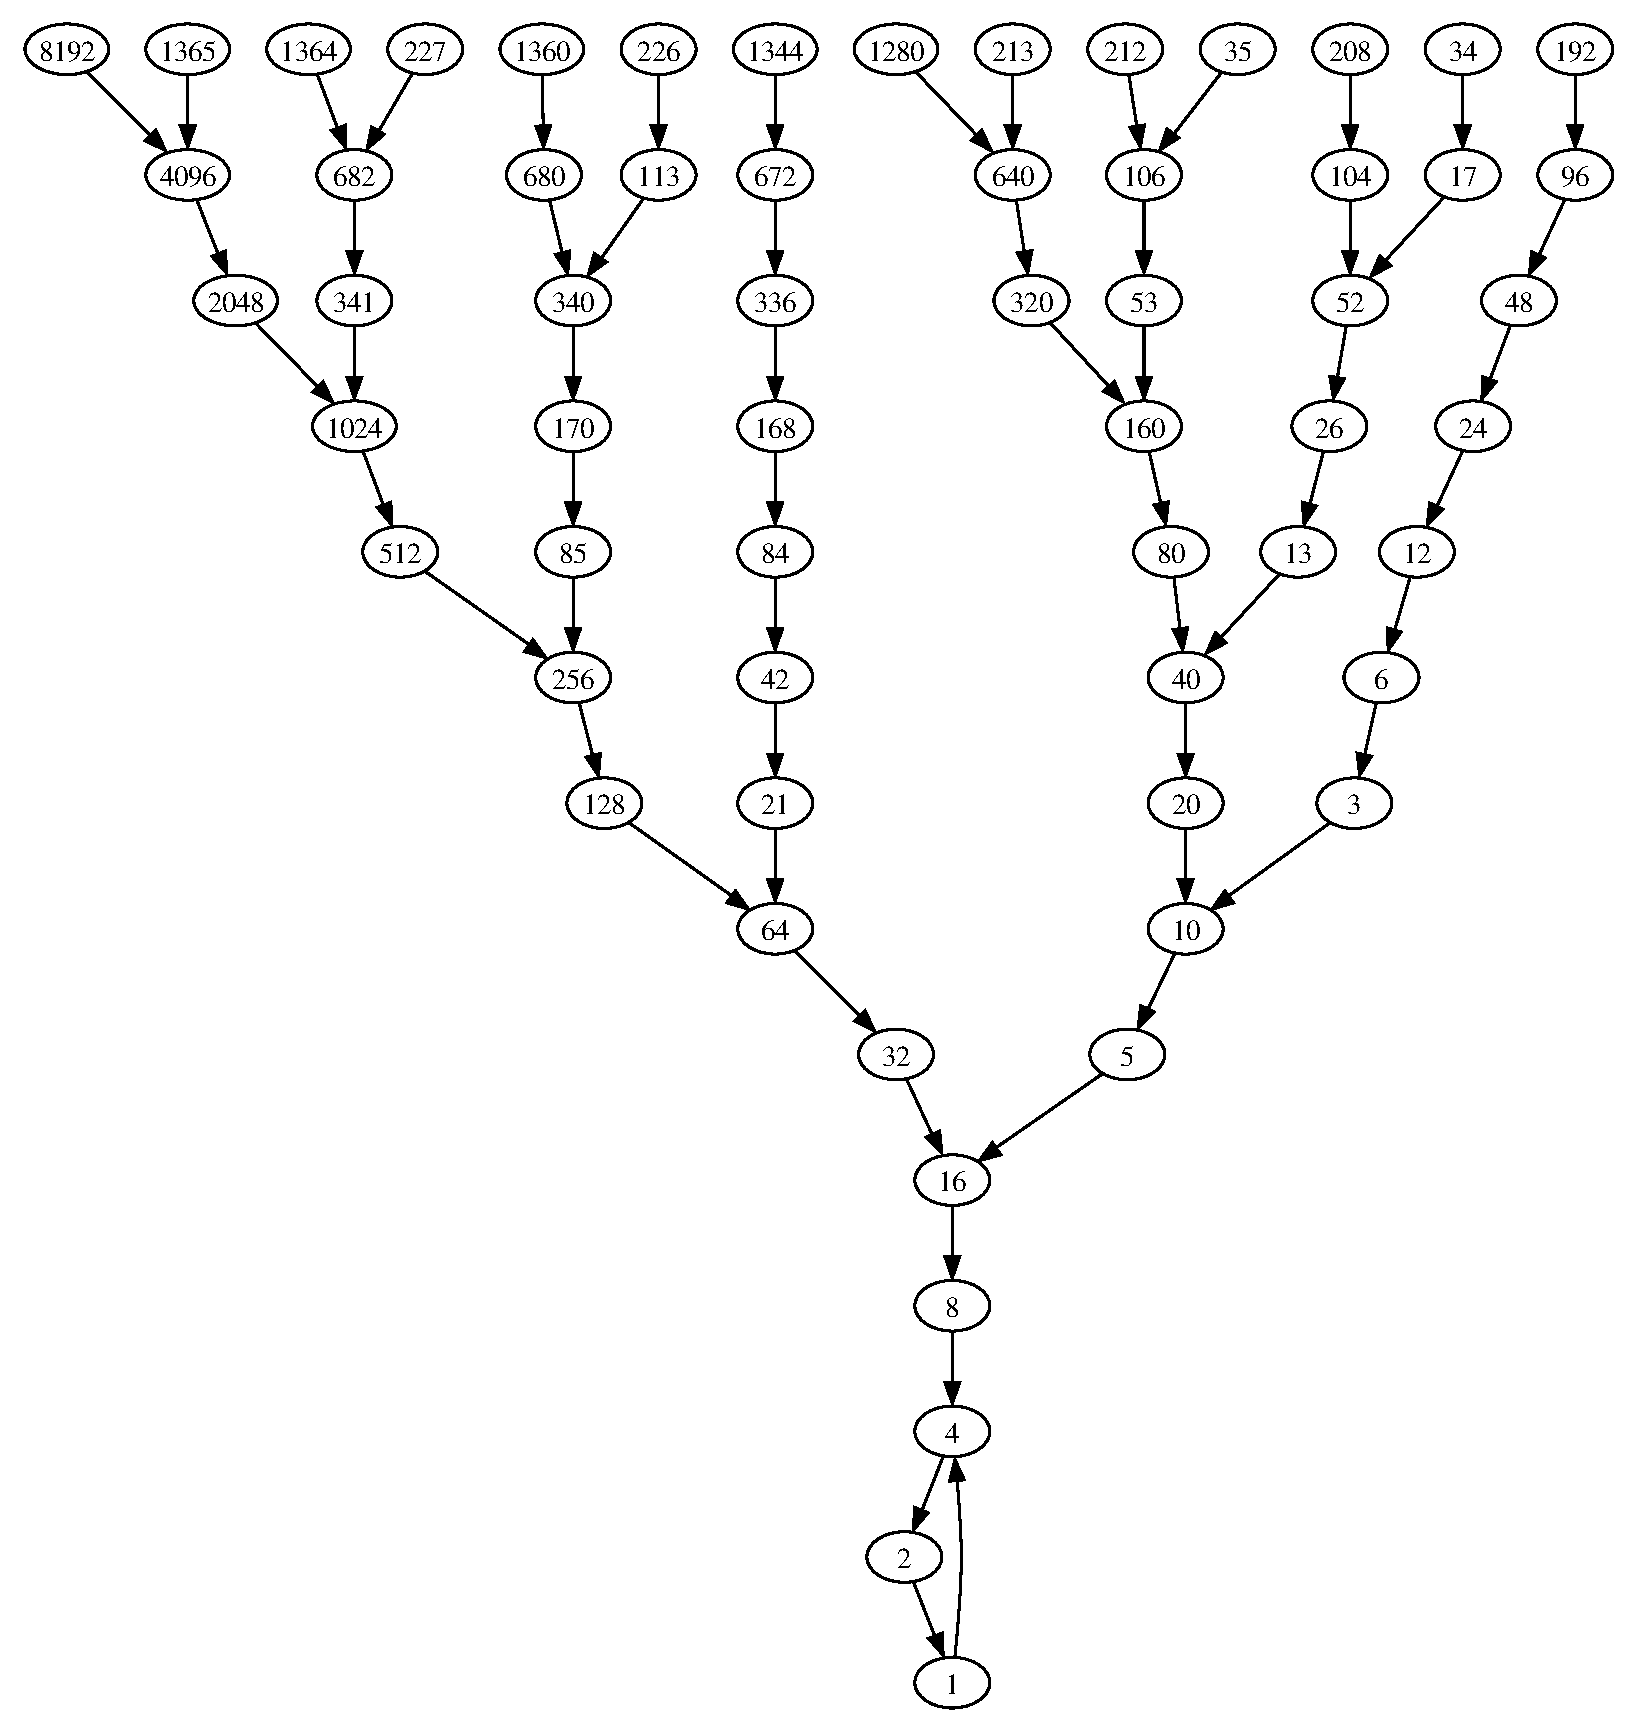
\includegraphics[width=.95\linewidth]{cgraph.eps}\par\nobreak
このグラフで, 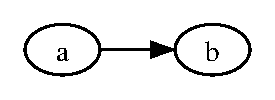
\includegraphics[width=2cm]{cgraphexample.eps}は$\func{c}(a)=b$を表す。
\end{section}
%
\begin{section}{fmのグラフ}
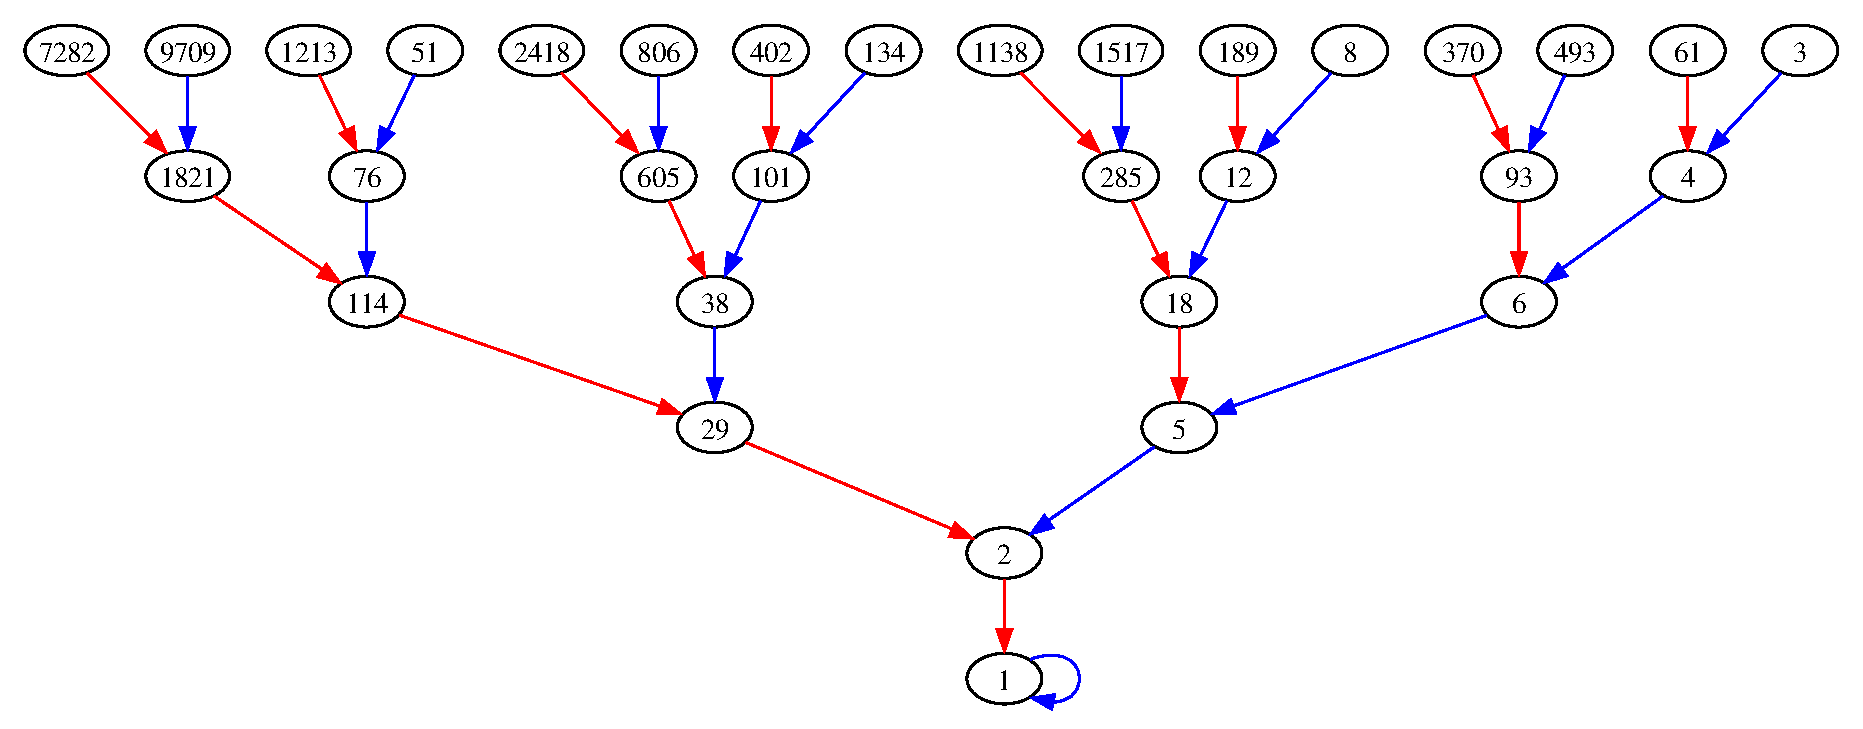
\includegraphics[width=.95\linewidth]{fmgraph.eps}\par\nobreak
このグラフで, 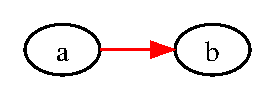
\includegraphics[width=2cm]{fmgraphexample1.eps}は$\func{fm}(a)=b\band\func{fminva}(b)=a$を, 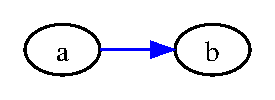
\includegraphics[width=2cm]{fmgraphexample2.eps}は$\func{fm}(a)=b\band\func{fminvb}(b)=a$を表す。
\end{section}
%
\begin{section}{fmのxyグラフ}
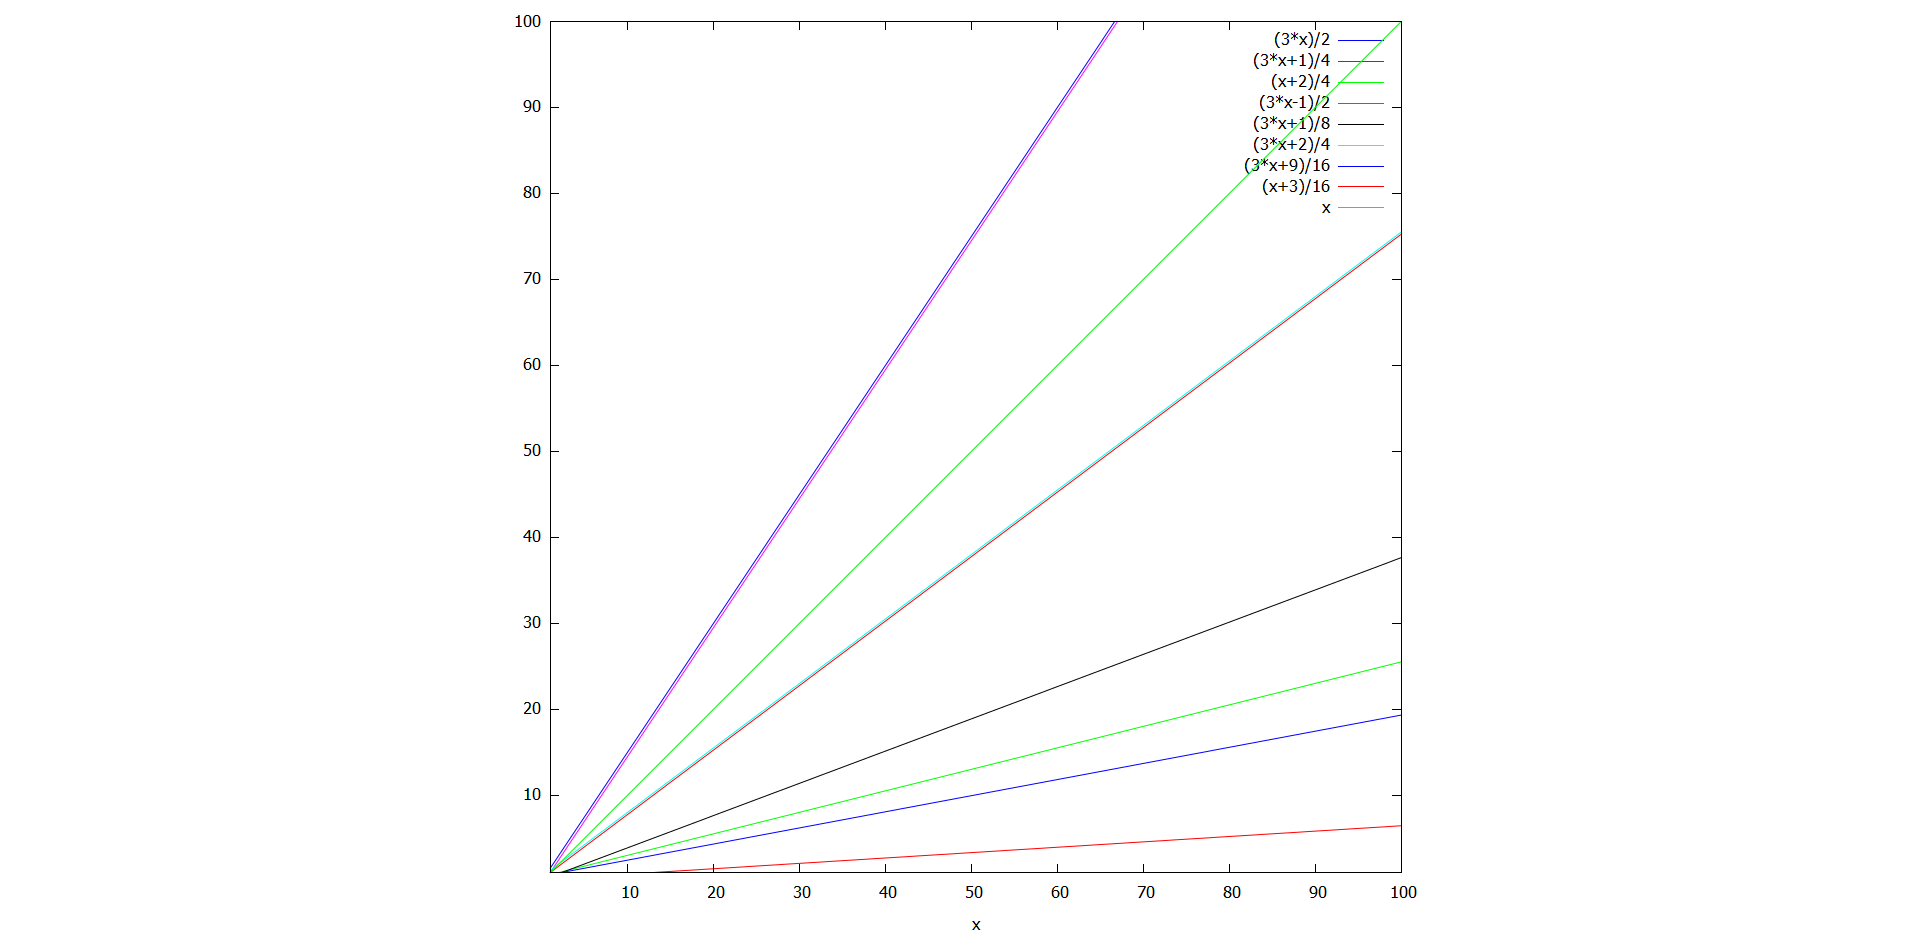
\includegraphics[width=.95\linewidth]{m32xymap.png}
\end{section}
%
\begin{section}{Maxima code}
\begin{samepage}
\begin{verbatim}
fm(j):=block(
    if mod(j,4)=0 then(
        return((3*j)/2)
    )
    elseif mod(j,8)=1 then(
        return((3*j+1)/4)
    )
    elseif mod(j,8)=2 then(
        return((j+2)/4)
    )
    elseif mod(j,4)=3 then(
        return((3*j-1)/2)
    )
    elseif mod(j,16)=5 then(
        return((3*j+1)/8)
    )
    elseif mod(j,8)=6 then(
        return((3*j+2)/4)
    )
    elseif mod(j,32)=13 then(
        return((3*j+9)/16)
    )
    else(
        return((j+3)/16)
    )
);
\end{verbatim}
\end{samepage}
\penalty0
\begin{samepage}
\begin{verbatim}
fminva(i):=block(
    if mod(i,2)=0 then(
        return(16*i-3)
    )
    else(
        return(4*i-2)
    )
);
\end{verbatim}
\end{samepage}
\penalty0
\begin{samepage}
\begin{verbatim}
fminvb(i):=block(
    if mod(i,6)=0 then(
        return((2*i)/3)
    )
    elseif mod(i,6)=1 then(
        return((4*i-1)/3)
    )
    elseif mod(i,6)=2 then(
        return((8*i-1)/3)
    )
    elseif mod(i,6)=3 then(
        return((16*i-9)/3)
    )
    elseif mod(i,6)=4 then(
        return((2*i+1)/3)
    )
    else(
        return((4*i-2)/3)
    )
);
\end{verbatim}
\end{samepage}
\penalty0
\begin{samepage}
\begin{verbatim}
fm_print(j):=block(
    if mod(j,4)=0 then(
        printf(true,"A"),
        return((3*j)/2)
    )
    elseif mod(j,8)=1 then(
        printf(true,"B"),
        return((3*j+1)/4)
    )
    elseif mod(j,8)=2 then(
        printf(true,"C"),
        return((j+2)/4)
    )
    elseif mod(j,4)=3 then(
        printf(true,"D"),
        return((3*j-1)/2)
    )
    elseif mod(j,16)=5 then(
        printf(true,"E"),
        return((3*j+1)/8)
    )
    elseif mod(j,8)=6 then(
        printf(true,"G"),
        return((3*j+2)/4)
    )
    elseif mod(j,32)=13 then(
        printf(true,"H"),
        return((3*j+9)/16)
    )
    else(
        printf(true,"I"),
        return((j+3)/16)
    )
);
\end{verbatim}
\end{samepage}
\penalty0
\begin{samepage}
\begin{verbatim}
fminva_print(i):=block(
    if mod(i,2)=0 then(
        printf(true,"J"),
        return(16*i-3)
    )
    else(
        printf(true,"K"),
        return(4*i-2)
    )
);
\end{verbatim}
\end{samepage}
\penalty0
\begin{samepage}
\begin{verbatim}
fminvb_print(i):=block(
    if mod(i,6)=0 then(
        printf(true,"L"),
        return((2*i)/3)
    )
    elseif mod(i,6)=1 then(
        printf(true,"M"),
        return((4*i-1)/3)
    )
    elseif mod(i,6)=2 then(
        printf(true,"N"),
        return((8*i-1)/3)
    )
    elseif mod(i,6)=3 then(
        printf(true,"O"),
        return((16*i-9)/3)
    )
    elseif mod(i,6)=4 then(
        printf(true,"P"),
        return((2*i+1)/3)
    )
    else(
        printf(true,"Q"),
        return((4*i-2)/3)
    )
);
\end{verbatim}
\end{samepage}
\penalty0
\begin{samepage}
\begin{verbatim}
mrank(k):=floor(k/6)+floor((k+7)/8)+floor((k+11)/16)
    +floor((k+14)/24)+floor((k+2)/6)+floor((k+2)/8);
\end{verbatim}
\end{samepage}
\end{section}
%
\begin{section}{C++ code}
\begin{samepage}
\begin{verbatim}
int fm(int j){
    if(j%4 == 0){
        return (3*j)/2;
    }
    else if(j%8 == 1){
        return (3*j+1)/4;
    }
    else if(j%8 == 2){
        return (j+2)/4;
    }
    else if(j%4 == 3){
        return (3*j-1)/2;
    }
    else if(j%16 ==5){
        return (3*j+1)/8;
    }
    else if(j%8 == 6){
        return (3*j+2)/4;
    }
    else if(j%32 == 13){
        return (3*j+9)/16;
    }
    else{
        return (j+3)/16;
    }
}
\end{verbatim}
\end{samepage}
\penalty0
\begin{samepage}
\begin{verbatim}
int fminva(int i){
    if(i%2 == 0){
        return 16*i-3;
    }
    else{
        return 4*i-2;
    }
}
\end{verbatim}
\end{samepage}
\penalty0
\begin{samepage}
\begin{verbatim}
int fminvb(int i){
    if(i%6 == 0){
        return (2*i)/3;
    }
    else if(i%6 == 1){
        return (4*i-1)/3;
    }
    else if(i%6 == 2){
        return (8*i-1)/3;
    }
    else if(i%6 == 3){
        return (16*i-9)/3;
    }
    else if(i%6 == 4){
        return (2*i+1)/3;
    }
    else{
        return (4*i-2)/3;
    }
}
\end{verbatim}
\end{samepage}
\end{section}
%
\end{document}
